\chapter{Cash-flow Analysis}

\section{Cash-flows}
\begin{definition}
    [Cash-flow]
    A \textit{cash-flow} is a series of cash receipts and payments, they can be positive or negative.
\end{definition}
\begin{itemize}
    \item First (Capital) Cost - the initial cost of an investment
    \item Revenues (Sales) - cash inflows from the sale of goods or services
    \item Operations and Maintenance (O\&M) - cash outflows for the operation and maintenance of the investment
    \item Overhaul and Replacement - cash outflows for the overhaul and replacement of the investment
    \item Salvage Value - cash inflows from the sale of the investment at the end of its useful life
    \item Scrap Value - cash inflows from the sale of the investment at the end of its useful life
    \item Disposal Cost - cash outflows for the disposal of the investment at the end of its useful life
\end{itemize}

\begin{definition}
    [Project Life-cycle Cost]
    Costs that occur at the start, during, or end of a project.
\end{definition}

\begin{figure}[H]
    \centering
    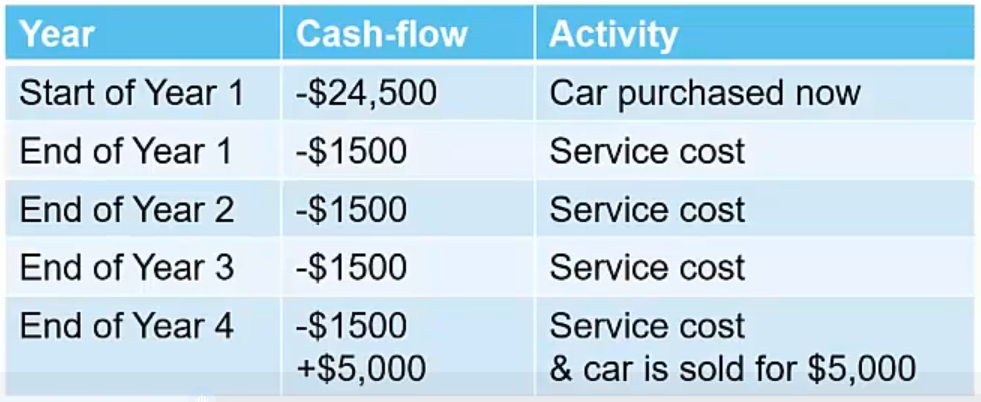
\includegraphics[width=0.8\textwidth]{LECTURE_2/cash-flow_table.png}
    \caption{Cash-flow Table}
    \label{fig:cash-flow_table}
\end{figure}

\begin{definition}
    [Cash-flow Diagram]
    A diagram that shows the cash-flows of a project over time.
    \begin{itemize}
        \item X-axis: time, Y-axis: cash-flow
        \item Y-axis: size and direction of cash-flow
        \item Individual cash-flows are shown as arrows
              \begin{itemize}
                  \item Upward arrows: cash inflows (disbursements)
                  \item Downward arrows: cash outflows (recipts)
              \end{itemize}
        \item Time 0 is the beginning of period 1
        \item Cash-flows occuring during a period is assumed to have occured at the end of that period
        \item Interest is compounded at the end of each period
    \end{itemize}
\end{definition}
\begin{figure}[H]
    \centering
    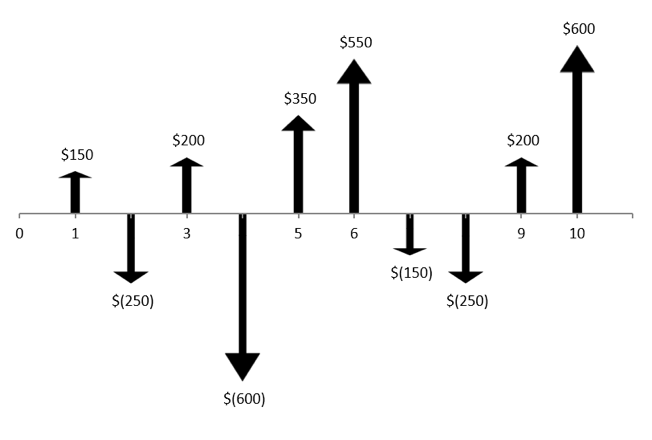
\includegraphics[width=0.8\textwidth]{LECTURE_2/cash-flow-diagram.png}
    \caption{Cash-flow Diagram}
    \label{fig:cash-flow_diagram}
\end{figure}

\begin{remark}
    Cash-flow diagrams from the lender's perspective is reversed from the borrower's perspective.
    % two side-by side diagrams
    \begin{figure}[H]
        \centering
        \begin{subfigure}[b]{0.4\textwidth}
            \centering
            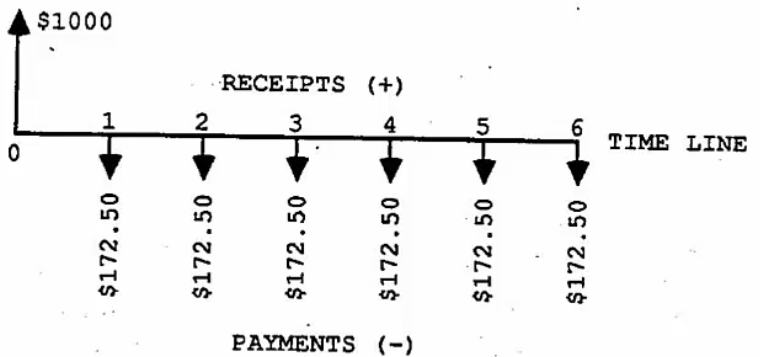
\includegraphics[width=\textwidth]{LECTURE_2/borrower_s_cash-flow.png}
            \caption{Borrower's Perspective}
            \label{fig:cash-flow_diagram_borrower}
        \end{subfigure}
        \begin{subfigure}[b]{0.4\textwidth}
            \centering
            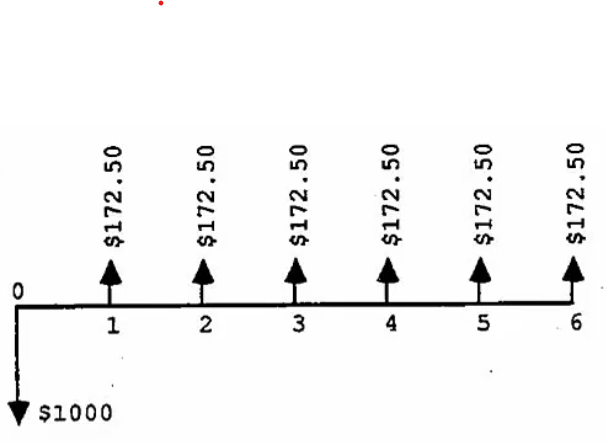
\includegraphics[width=\textwidth]{LECTURE_2/lender_s_cash-flow.png}
            \caption{Lender's Perspective}
            \label{fig:cash-flow_diagram_lender}
        \end{subfigure}
        \caption{Cash-flow Diagrams}
        \label{fig:cash-flow_diagrams}
    \end{figure}
\end{remark}

\begin{example}
    Young Professional: Çonstruct a cash-flow diagram with the
    following cash-flows (assume 4 weeks per month)
    $\cdot$ Monthly income:  \$ 2200( received at the end of each' month)
    Rent includes utilities: \$700 (at the end of each month)
    Weekly food and entertainment: \$120
    Telephone bill: \$40 (at the end of the first week of each month)
    Credit card purchases: \$300 (at the end of the second week of each
    month)
    \begin{figure}[H]
        \centering
        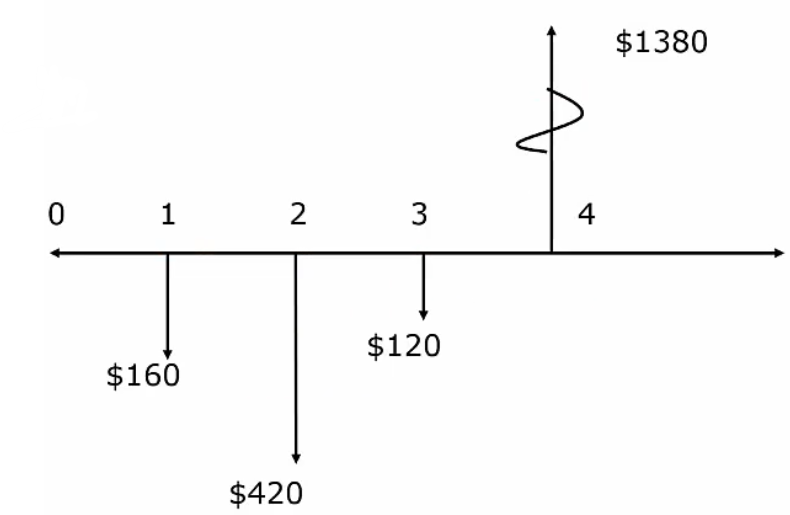
\includegraphics[width=0.8\textwidth]{LECTURE_2/cash-flow-ex.png}
        \caption{Young Professional Cash-flow Diagram}
        \label{fig:young_professional_cash-flow}
    \end{figure}
\end{example}

\section{Cash-flow Categories}

\begin{definition}
    [Single Payments/ Receipts]
    Cash-flows that occur only once.
\end{definition}

\begin{definition}
    [Perpetuity]
    Cash-flows that occur indefinitely.
\end{definition}
\begin{figure}[H]
    \centering
    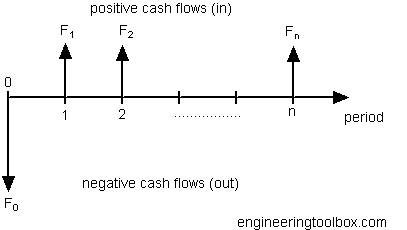
\includegraphics[width=0.8\textwidth]{LECTURE_2/perpetuity.png}
    \caption{Perpetuity Cash-flow Diagram ($n \to \infty$)}

\end{figure}

\begin{definition}
    [Annuity]
    Cash-flows that occur at regular intervals (e.g. coupon payments, bonds, etc.)
\end{definition}
\begin{figure}[H]
    \centering
    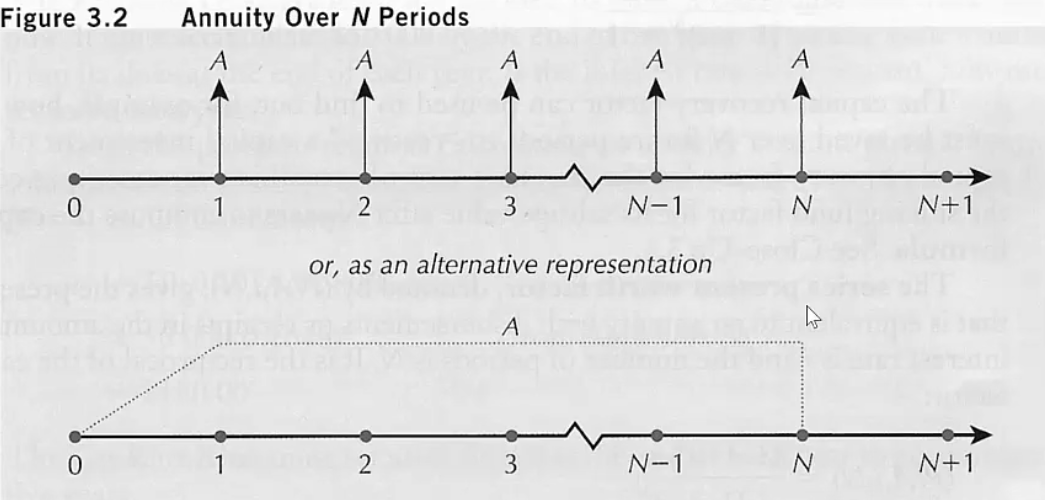
\includegraphics[width=0.8\textwidth]{LECTURE_2/annuity.png}
    \caption{Annuity Cash-flow Diagram}
    \label{fig:annuity_cash-flow}
\end{figure}

\begin{definition}
    [Arithmetic Gradient]
    Cash-flows that increase or decrease by a constant amount at regular intervals.
    \begin{equation}
        A_n = A' + (N-1)G
    \end{equation}
    Where:
    \begin{itemize}
        \item $A'$ is the original amount
        \item $G$ is the amount added
        \item $N$ is the number of periods
    \end{itemize}
\end{definition}
\begin{figure}[H]
    \centering
    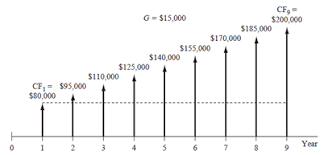
\includegraphics[width=0.8\textwidth]{LECTURE_2/arithmetic_gradient.png}
    \caption{Arithmetic Gradient Cash-flow Diagram}
    \label{fig:arithmetic_gradient_cash-flow}
\end{figure}

\begin{definition}
    [Geometric Gradient]
    Cash-flow that grows exponentially such that if $A$ is the principal cash-flow, then the cash-flow at period $N$ is $A_N = A(1+g)^{N-1}$
\end{definition}

\begin{figure}[H]
    \centering
    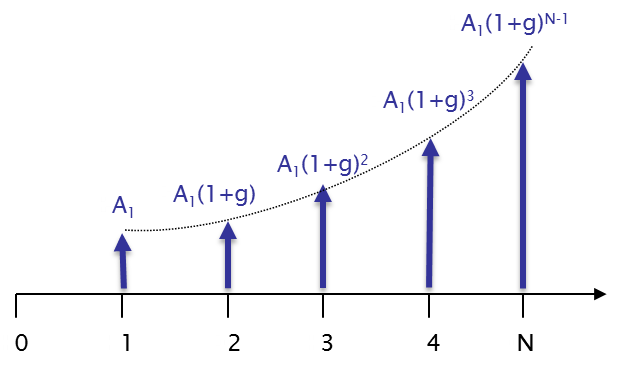
\includegraphics{LECTURE_2/geometric-gradient-series.png}
    \caption{Geometric Cash-flow Diagram}
    \label{geom-cash-flow}
\end{figure}

\section{Cash-flow Equivalence}

\subsection{Mathematical Equivalence}
\begin{definition}
    [Mathematical Equivalence]
    Two cash-flows, $P_t$ at time $t$ and $F_{t+N}$ at time $t+N$ are mathematically equivalent if, at a certain interest rate $i$, they have the same present value or future value:
    \[
        F_{t+N} = P_t(1+i)^N
    \]
    \textit{If the time changes, the magnitude of the cash-flow changes accordingly.}
\end{definition}

\begin{figure}[H]
    \centering
    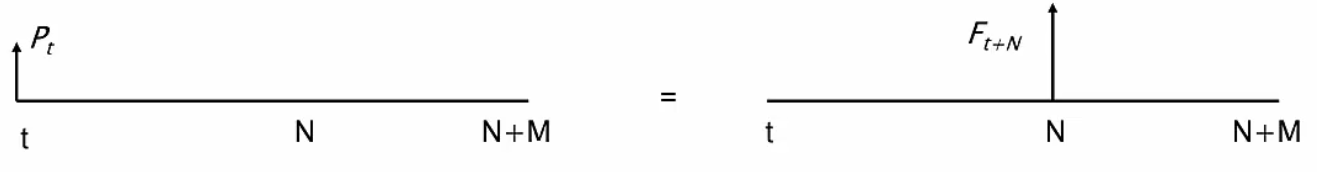
\includegraphics[width=0.8\textwidth]{LECTURE_2/mat-equiv.png}
    \caption{Mathematical Cash-flow Diagram}
    \label{fig:mathematical_cash-flow}
\end{figure}

\begin{definition}
    [Market Equivalence]
    The ability to exchange cash-flows in the market without any loss. \\
    \begin{itemize}
        \item Exchanging $P_t$ for $F_{t+N}$ at time $t$ is lending money.
        \item Exchanging $F_{t+N}$ for $P_t$ at time $t$ is borrowing money.
    \end{itemize}
\end{definition}

\begin{example}
    [Treasury Bills]
    A Treasury Bill(T-bill) is a short-term government debt obligation backed by the government with a maturity of one year or less. T-bills are usually sold in denominations of $\$1,000$. If a $\$1000$ T-bill due to mature in 6 months is currently selling for $\$990.10$ then that means some investors holding the Tbill are willing to sell them at this price while others are willing to buy them at this price. The“market” has agreed that the appropriate interest rate is 1\% over 6 months. Confirm this by calculating the yield.
    \begin{align*}
        FV   & = \$1000                      \\
        PV   & = \$990.10                    \\
        N    & = 0.5 \text{ years}           \\
        i    & = ?                           \\
        FV   & = PV(1+i)^N                   \\
        1000 & = 990.10(1+i)^{0.5}           \\
        1+i  & = {\frac{1000}{990.10}}^2     \\
        i    & = {\frac{1000}{990.10}}^2 - 1 \\
        i    & \approx 0.01
    \end{align*}
\end{example}

\begin{definition}
    [Decisional Equivalence]
    The indifference of an investor to choose between two cash-flows, e.g. $P_t$ at time $t$ and $F_{t+N}$ at time $t+N$.
\end{definition}

\begin{example}
    \begin{itemize}
        \item Need: 1,000 kg aluminium on August 15
        \item Offer: 1,100 kg aluminium on August 22
        \item Same price and payment at the end of August
        \item An implied interest rate offer of 10\% for a week
    \end{itemize}
    The question is: How much is it worth for decision maker to accept the delay in delivery? \\
    If the manufacturer has a lot of aluminum in stock, it may be worth it to wait a week to get the extra 100 kg. If the manufacturer is running low on aluminum, the manufacturer may have to pay in penalties, or pay workers over-time to meet the deadline.
\end{example}



\section{Cash-flow Factors}

\begin{theorem}
    [Factor Notation]
    \begin{itemize}
        \item $(X/Y, i, N)$ - the factor that converts one kind of cash-flow to another
              \begin{itemize}
                  \item $X$ and $Y$ are one of the following:
                        \begin{itemize}
                            \item $F$ - future value
                            \item $P$ - present value
                            \item $A$ - annual value
                            \item $G$ - gradient
                            \item $g$ - growth rate
                        \end{itemize}
                  \item So, to convert from a present value $P$ to a future value $F$ at interest rate $i$ for $N$ periods, we use the factor $(P/F, i, N)$, which is read as "P given F at i for $N$ periods"
                  \item For the geometric gradient, we use $P = (P/G, i, g, N)$
              \end{itemize}
        \item Some factors have specific names
              \begin{itemize}
                  \item $(F/P, i, N)$ - Compound amount factor
                  \item $(P/F, i, N)$ - Present worth factor
                  \item $(A/F, i, N)$ - Sinking fund factor
                  \item $(F/A, i, N)$ - Series compound amount factor
                  \item $(A/P, i, N)$ - Capital recovery factor
                  \item $(P/A, i, N)$ - Series present worth factor
              \end{itemize}
    \end{itemize}
\end{theorem}

\begin{corollary}
    [Compound Amount Factor]
    \[
        F = P(1+i)^N
    \]
    \[
        (F/P, i, N) = (1+i)^N
    \]
\end{corollary}

\begin{example}
    If you had \$2000 now and invested it at 10\% interest, how much would you have in 8 years? \\
    \textbf{Solution:}
    \begin{align}
        P & = 2000, i = 0.1, N = 8 \\
        F & = P(P/F, i, N)         \\
        F & = 2000(P/F, 10\%, 8)   \\
        F & = 2000(1+0.1)^8        \\
        F & = 2000(2.143)          \\
        F & = 4287.20
    \end{align}
\end{example}
\begin{definition}
    [Present Worth Factor]
    \begin{align}
        P           & = \frac{F}{(1+i)^N} \\
        (P/F, i, N) & = \frac{1}{(1+i)^N} \\
        (F/P, i, N) & = (1+i)^N
    \end{align}
\end{definition}

\begin{definition}
    [Discount Rate]
    The interest rate used to convert future cash-flows to present value.\\
    For example, if you invest \%100 at 5\% interest, you expect to have $F = P \times (1+i) = \$100\times(1.05) = \$105$ at the end of the year. Therefore:
    \[
        P = \frac{F}{(1+i)^N} \qquad i \text{ is the discount rate, $N$ is the number of periods}
    \]
\end{definition}

\begin{definition}
    [Present Value of a Perpetuity]
    \begin{align}
        P & = \frac{A}{1 + i} + \frac{A}{(1+i)^2} + \frac{A}{(1+i)^3} + \ldots = \frac{A}{i}
    \end{align}
\end{definition}

\begin{definition}
    [Present Value of an Annuity]
    The present value of an annuity is equal to a perpetuity starting at the first period minus a perpetuity of the same size starting at the $N+1$ period.
    \begin{align}
        P          & = A(P/A, i, N) = P_1 - P_2                                  \\
        P_1        & = \frac{A}{i}                                               \\
        P_2        & = \frac{A}{i}(1+i)^{-N}                                     \\
        P          & = A(\frac{1}{i} - \frac{1}{i}(1+i)^{-N})                    \\
        \therefore & \boxed{(P/A, i, N) = \frac{1}{i}( 1 - \frac{1}{(1+i)^{N}})}
    \end{align}
    \textit{Note: The second annuity, like all annuities, is also worth $A/i$, but because it starts at the $N+1$ period, we discount it.}
\end{definition}


\begin{definition}
    [Present Value of an Arithmetic Growth Factor]
    The arithmetic gradient is the sum of $N$ annuities, each increasing by a constant amount $G$. Remember that arithmetic gradients begin at period 1.
    \begin{align*}
        P           & = G(P/G, i, N) =                                                                                                                                                           \\
        P           & = G \left(\frac{(P/A, i, n-1)}{1 + i} + \frac{(P/A, i, n-2)}{(1 + i)^2} + \cdots + \frac{(P/A, i, 1)}{(1+i)^{n-1}}\right)                                                  \\
        \rightarrow & \quad \text{remember that } (P/A, i, N) = \frac{1}{i}\left(1 - \frac{1}{(1+i)^a}\right)                                                                                    \\
        P           & = \frac{G}{i} \left(
        \frac{1}{1+i} + \frac{1}{(1+i)^2} + \cdots + \frac{1}{(1+i)^{N-1}}
        \right)                                                                                                                                                                                  \\
                    & + \frac{G}{i} \left(
        - \frac{1}{(1+i)}\frac{1}{(1+i)^{N-1}} - \frac{1}{(1+i)^2}\frac{1}{(1+i)^{N-2}} - \cdots - \frac{1}{(1+i)^{N-1}}\frac{1}{1}
        \right)                                                                                                                                                                                  \\
        \rightarrow & \text{ The first term resembles an annuity, so we can add $\frac{1}{(1 + i)^N}$ to complete it}                                                                            \\
        P           & = \frac{G}{i}\left(                                    \frac{1}{1+i} + \frac{1}{(1+i)^2} + \cdots + \frac{1}{(1+i )^N} - \frac{1}{(1+i)^N} - \frac{n -1}{(1 + i)^N}\right)
        \\
        P           & = \frac{G}{i}\left(\frac{1}{i}(1 - \frac{1}{(1 + i)^N}) - \frac{N}{(1 + i)^N}\right)                                                                                       \\
        P           & = \frac{G}{i^2}\left(1 - \frac{1+iN}{(1 + i)^N}\right)                                                                                                                     \\
        \therefore  & \boxed{(P/G, i, N) = \frac{1}{i^2}\left(1 - \frac{1+iN}{(1 + i)^N}\right)}
    \end{align*}
    \textit{Note: To get the total arithmetic gradient present value, add the growth factor to the initial annuity such that: $P = A(P/A, i, N) + G(P/G, i, N)$}
\end{definition}

\begin{definition}
    [Present Value of a Geometric Gradient]
    Looking at the figure \ref{geom-cash-flow}, we can model the present value of a geometric gradient, keeping in mind to discount the cash-flows at the end of each period.
    \begin{align*}
        P           & = \frac{A}{1 + i} + \frac{A(1+g)}{(1+i)^2} + \ldots + \frac{A(1+g)^{N-1}}{(1+i)^N}                                   \\
        P           & = \frac{A}{1 + g}\left(
        \frac{1 + g}{1 + i} + \frac{(1 + g)^2}{(1 + i)^2} + \ldots + \frac{(1 + g)^{N}}{(1 + i)^{N}}
        \right)                                                                                                                            \\
        \rightarrow & \text{ Let's define } \frac{1}{1 + i^0} = \frac{1+g}{1+i} \iff i^0 = \frac{1 + i}{1 + g} -1                          \\
        P           & = \frac{A}{1 + g} ( \frac{1}{1 + i^0} + \frac{1}{(1 + i)^2} + \ldots + \frac{1}{(1 + i)^N})                          \\
        \rightarrow & \text{ We can use the present value of an annuity to simplify this}                                                  \\
        P           & = \frac{A}{1 + g} (P/A, i^0, N)                                                                                      \\
        P           & = A \times \frac{1 - (\frac{1 + g}{1 + i})^N}{i - g}                                                                 \\
        \therefore  & \boxed{(P/G, i, g, N) =\begin{aligned}
                                                                & \frac{1 - (\frac{1 + g}{1 + i})^N}{i - g}                                     \\
                                                     \text{or } & \frac{(P/A, i^0, N)}{1 + g} \quad \text{where } i^0 = \frac{1 + i}{1 + g} - 1
                                                 \end{aligned}}
    \end{align*}
\end{definition}

\section{Examples Using Cash-flow Factors}
\begin{example}
    [The Magic of Compound Interest]
    If you are 20 years old and save and invest \$1.00 each day, assume you live to age 80 and the annual interest rate is 10\%, you can become a millionaire! Let's verify
    \textbf{Solution:}
    First convert annual interest to daily interest:
    \begin{align}
        (1 + r)^365&  = 1 + 0.1 \\
        r          & = 0.02612\% \\
        F = \$ 1 \times (A/F, 0.02612\%, 60 \times 365) \\
        & = \$ 1 \times (F/P, 0.02612\%, 60 \times 365)\times (A/F, 0.02612\%, 60 \times 365) \\
        & = \$ 1.162 M\\
    \end{align}
\end{example} 

\begin{theorem}
    [Compounded Interest Rates]
    A yearly interest rate $r$ compounded $m$ times per year is equivalent to an interest rate $i_s = \frac{r}{m}$ per subperiod, such that:
    \begin{align}
        F & = P(1 + \frac{r}{m})^{mN} \\
        F & = P(F/P, \frac{r}{m}, mN)
    \end{align}
\end{theorem}
% \chapter{Lecture Problems}

% \begin{example}
%     Consider Annuity that pays $\$10$ per month for 1 year. If interest is $1\%$ per month, compounded monthly. What is the equivalent continuous payment rate? \\
%     \textbf{Solution:}
%     \begin{align}
%         P   & = \$10 (p/A, 1\%, 12) = \$112.56 \\
%         P_0 & = A\int_0^1 e^{r_{cc}t} dt       \\
%         P_0 & = A\int_0^1 e^{0.01t} dt         \\
%         r   & = 11.94\% / \text{year}
%     \end{align}
% \end{example}

% \begin{example}
%     Determine the effective annual rate for an investment that earns $15\%$ per year based on
%     quarterly compounding for the first $4$ months, then earns $11\%$ per year based on continuous
%     compounding for another $5$ months.
% \end{example}

